\documentclass[a4paper,12pt]{article}
\usepackage{amssymb} % needed for math
\usepackage{amsmath} % needed for math
\usepackage[utf8]{inputenc} % this is needed for german umlauts
\usepackage[ngerman]{babel} % this is needed for german umlauts
\usepackage[T1]{fontenc}    % this is needed for correct output of umlauts in pdf
\usepackage[margin=2.5cm]{geometry} %layout
\usepackage{booktabs}
\usepackage{lmodern}

% this is needed for forms and links within the text
\usepackage{hyperref}

% glossar, see http://en.wikibooks.org/wiki/LaTeX/Glossary
% has to be loaded AFTER hyperref so that entries are clickable
\usepackage[nonumberlist]{glossaries}

% The following is needed in order to make the code compatible
% with both latex/dvips and pdflatex.
\ifx\pdftexversion\undefined
\usepackage[dvips]{graphicx}
\else
\usepackage[pdftex]{graphicx}
\DeclareGraphicsRule{*}{mps}{*}{}
\fi

\makeglossaries

%%%%%%%%%%%%%%%%%%%%%%%%%%%%%%%%%%%%%%%%%%%%%%%%%%%%%%%%%%%%%%%%%%%%%%
% Variablen                                 						 %
%%%%%%%%%%%%%%%%%%%%%%%%%%%%%%%%%%%%%%%%%%%%%%%%%%%%%%%%%%%%%%%%%%%%%%
\newcommand{\authorName}{uuoof}
\newcommand{\auftraggeber}{Karlsruhe Institute of Technology (Teco)}
\newcommand{\auftragnehmer}{wir}
\newcommand{\projektName}{Earables}
\newcommand{\tags}{\authorName, Pflichtenheft, KIT, Informatik, PSE}
\newcommand{\glossarName}{Glossar}
\title{\projektName~(Pflichtenheft)}
\author{\authorName}
\date{\today}

%%%%%%%%%%%%%%%%%%%%%%%%%%%%%%%%%%%%%%%%%%%%%%%%%%%%%%%%%%%%%%%%%%%%%%
% PDF Meta information                                 				 %
%%%%%%%%%%%%%%%%%%%%%%%%%%%%%%%%%%%%%%%%%%%%%%%%%%%%%%%%%%%%%%%%%%%%%%
\hypersetup{
  pdfauthor   = {\authorName},
  pdfkeywords = {\tags},
  pdftitle    = {\projektName~(Pflichtenheft)}
}

%%%%%%%%%%%%%%%%%%%%%%%%%%%%%%%%%%%%%%%%%%%%%%%%%%%%%%%%%%%%%%%%%%%%%%
% Create a shorter version for tables. DO NOT CHANGE               	 %
%%%%%%%%%%%%%%%%%%%%%%%%%%%%%%%%%%%%%%%%%%%%%%%%%%%%%%%%%%%%%%%%%%%%%%
\newcommand\addrow[2]{#1 &#2\\ }

\newcommand\addheading[2]{#1 &#2\\ \hline}
\newcommand\tabularhead{\begin{tabular}{lp{13cm}}
\hline
}

\newcommand\addmulrow[2]{ \begin{minipage}[t][][t]{2.5cm}#1\end{minipage}%
   &\begin{minipage}[t][][t]{8cm}
    \begin{enumerate} #2   \end{enumerate}
    \end{minipage}\\ }

\newenvironment{usecase}{\tabularhead}
{\hline\end{tabular}}

\usepackage{microtype}


%%%%%%%%%%%%%%%%%%%%%%%%%%%%%%%%%%%%%%%%%%%%%%%%%%%%%%%%%%%%%%%%%%%%%%
% THE DOCUMENT BEGINS             	                              	 %
%%%%%%%%%%%%%%%%%%%%%%%%%%%%%%%%%%%%%%%%%%%%%%%%%%%%%%%%%%%%%%%%%%%%%%
\begin{document}
 \pagenumbering{roman}
 \begin{titlepage}
\maketitle
\thispagestyle{empty} % no page number

\begin{verbatim}












\end{verbatim}


  \begin{tabular}[t]{p{4 cm}p{8 cm}}
	Projekt:       & \projektName \\[1.2ex]
	Auftraggeber:  & \auftraggeber\\[1.2ex]
	Auftragnehmer: & \auftragnehmer\\[1.2ex]
  \end{tabular}


\begin{tabular}[t]{|p{4 cm}|p{8 cm}|}
\hline
\textbf{Datum} & \textbf{Autor(en)} \\
\hline
\hline
\today & \authorName \\
\hline
\end{tabular}
\end{titlepage}
         % Deckblatt.tex laden und einfügen
 \setcounter{page}{2}
 \tableofcontents          % Inhaltsverzeichnis ausgeben
 \clearpage
 \pagenumbering{arabic}

\section{Einleitung}
Earables gehören zu den Wearable Computings. Sie sind also nichts anderes als intelligente Kopfhörer. Je nach dem wie sie ausgestattet werden bringen sie die unterschiedlichsten Funktionen mit sich. Neben der klassischen Austattung von  Lautsprechern, Mikrophon und Bluetooth Low Energy besitzen sie in unserem Fall zusätzlich ein 6-Achsen IMU (Beschleunigungssensor und Gyroskop) . Mit seiner Hilfe ist man in der Lage die (Kopf-)Bewegung des Nutzers zu tracken um mit den gewonnenen Messdaten  beispielsweise die Atemfrequenz zu ermitteln. Earebles bilden also eine Schnittstelle von Mensch und Computer. Mit ihnen kann man unauffällig medizinische Daten im Altag sammeln. Da sie kaum von normalen Bluetooth Kopfhörern zu unterscheiden sind haben sie bereits ein hohe soziale akzeptans in der Gesellschaft erlangt, im Gegensatz zu beispielsweise den smart Glasses. Mit der Entwicklung und Forschung dieser Art von Earables beschäftigt sich das globale eSense Projekt von Nokia Bell Labs in Zusammenarbeit mit dem Telecooperation Office (TECO). Hier wird gemeinsam nach möglichen Anwendungsfällen der Earables gesucht, wodurch auch dieses Projekt seinen Weg in diese Welt gefunden hat.
\section{Zielbestimmung}
Die Ziele dieses Projektes lassen sich in drei Bereiche gliedern:
\begin{enumerate}

  \item Es soll eine Cross-Plattform Bibliothek (Android/IOS) für die Earables der Plattform eSense entwickelt werden mit der es möglich ist, die Messdaten des Gerätes aufzuzeichnen und verschiedene Steuerungsparameter zu verändern.
  
  \item Es soll ein Erweiteungsmodul entwickelt werden, mit der es Möglich ist gewisse Daten der Kopf auszuwerten, beispielsweise ob der Nutzer gerade läuft oder steht.
  
  \item %%app todo

\end{enumerate}

\subsection{Musskriterien}
%%bitte stichpunkte
Das Ziel der Bibliothek ist es, Kern-Funktionen zu beinhalten, um Messdaten auzulesen und die Steuerungsparameter zu verändern. Besonders wichtig ist, dass man in der Lage sein soll die Daten des 6-Achsen IMU auzulesen. Bezüglich des Erweiterungsmoduls soll es in der Lage sein zu erkennen ob der Nutzer gerade läuft oder steht und dies, über eine ansprechende GUI, auszugeben. Außerdem soll die GUI so benutzerfreundlich gestaltet werden, so dass der Benutzer intuitiv weiß wie man die Steuerungsparameter der Earables verändern kann.
\subsection{Wunschkriterien}
%%bitte stichpunkte
Als Wunschkriterium soll die App die Schrittfrequenz des Nutzers anzeigen und das im besten Fall in Echtzeit. Mit einer kurzen Verzögerung von ein paar Sekunden wird jedoch gerechnet. Zusätzlich soll die Anzahl der Schritte ausgegeben werden wodurch man die zurückgelegten Distanz ermitteln kann. Diese wird ebenfalls ausgegeben. Des weiteren sind 3 verschiedene Modi geplant. Im Modus „Counter“ zählt die App wie viele Liegestützen oder Sit Ups der Nutzer macht. Über den Modus „Listen and Perform“ ist der Nutzer in der Lage seinen eigenen Trainingsplan individuell für sich zu erstellen. Dieser wird dann, mit Hilfe von Text to Speech ausgegeben. Im letzten Modus Namens „Musik Run“ wird die Musik automatisch gestoppt, wenn der Nutzer steht und wieder gestartet, sobald der Nutzer damit beginnt weiter zu laufen. Die App wird auf deutsch sein, aber der Nutzer kann weitere Sprachen durch Sprachpaket-Plugins hinzufügen. Zum Abschluss soll es für den Nutzer möglich sein seine Trainingsdaten zu speichern, importieren und exportieren, um so mehrere „Projekte“ anzulegen.
  \subsection{Abgrenzungskriterien}
  %%bitte stichpunkte
Was wir nicht umsetzen wollen ist die Speicherung von Rohdaten, da dies zur Folge haben könnte, dass sich einige Nutzer ausspioniert fühlen. Generell wird die Speicherung von Daten nur auf dem Smartphone erfolgen und nicht auf dem Speicher der Earables. Das Ziel, die Geschwindigkeit der Musik an die Schrittfrequenz des Nutzers anzupassen, wird nicht verfolgt. Im Modus Liegestützen oder Sit Ups zählen wird davon ausgegangen, dass der Nutzer wirklich nur Liegestützen oder Sit Ups macht und nicht versucht das System auszutricksen.

% Was will ich bewusst nicht umsetzen?
% Was soll es nicht sein?

\section{Produkteinsatz}
  \subsection{Zielgruppe}
  \begin{itemize}
    \item\textsf{Bibliothek:} Softwareentwickler
    \item\textsf{Erweiterungsmodul:} Softwareentwickler
    \item\textsf{App:} Hobbysportler
  \end{itemize}
  \subsection{Anwendungsbereiche}
    \begin{itemize}
      \item\textsf{Bibliothek} Softwareentwicklung für eSense Wearables
      \item\textsf{Erweiterungsmodul} Softwareentwicklung im Bereich Schritterkennung
      \item\textsf{App} Heimtraining, Sport,\dots
    \end{itemize}
  \subsection{Betriebsbedinugen}
  TODO
    \begin{itemize}
      \item\textsf{Bibliothek} 
      \item\textsf{Erweiterungsmodul}
      \item\textsf{App}
    \end{itemize}

\section{Produktumgebung}
\subsection{Hardware} \textsf{Minimale Anforderungen:} Smartphone mit Bluetooth LE Unterstützung.
\subsection{Software} \textsf{Betriebssystem:} Android > 8.0 und iOS > 12.0

\section{Funktionale Anforderungen}
TODO Valle Koordination
% Was soll das Produkt machen können

  \subsection{Mussanforderungen}
  TODO alle: Man sollte hier funktionale Anforderungen \textbf{angeben und ergänzen}. Dabei nummeriert man in 10er Schritten.
    \subsubsection{Bibliothek}
    \begin{itemize}
      \item[/F010/] Daten des Gyroskops auslesen und in Echtzeit zur Verfügung stellen.
      \item[/F020/] Daten des Beschleunigungssensors auslesen und in Echtzeit zur Verfügung stellen.
      \item[/F030/] Messparameter (Abtastrate etc.) ändern. %%konkreter: Abtastrate (oder ???)
      \item[/F040/] Datenaufnahme des IMU starten und stoppen.
      \item[/F050/] BLE Charakteristiken unterstützen %%besprechen!!!
    \subsubsection{Erweiterungsmodul}
     Auswertung der ausgelesenen Daten:
      \item[/F060/] Schritterkennung (Stehen/Laufen des Nutzers).
    \subsubsection{App}
    %%TODO valle Glossareintrag Vorgang: "aktiv in modus"
      %%alles kürzer schreiben, nur je 1 Stichpunkt
      \item[/F070/] \textsf{App starten:} Der Nutzer kann die App über sein Smartphone starten. %%weglassen? Startbildschirmanzeige?
      \item[/F080/] \textsf{Modus auswählen:} Auswahl eines Modus aus allen verfügbaren Modi (also mindestens der Modus \glqq Laufen/Stehen anzeigen\grqq). 
      \item[/F090/] \textsf{Modus wechseln:} Wechseln zwischen Modi während ein Modus aktiv ist. %%aktueller Modus stoppt, nichtfunktionale Anforderung? 
      \item[/F100/] \textsf{Laufmodus:} Liveanzeige, ob Nutzer gerade \glqq läuft\grqq{} oder \glqq steht\grqq{}.
      \item[/F110/] \textsf{Vorgang starten:} Der Nutzer kann den modusspezifischen Vorgang starten. Dann wird der Modus nach seiner Beschreibung aktiv ausgeführt. Dies gilt für jeden Modus außer den Modus \glqq Livedaten\grqq.
      \item[/F120/] \textsf{Vorgang stoppen:} Der Nutzer kann den modusspezifischen Vorgang stoppen.
      \item[/F130/] \textsf{Resultat anzeigen:}Nach Stoppen Anzeigen des Vorgansresultats bis neuer Vorgang gestartet wird.
  \subsection{Wunschanforderungen}
    \subsubsection{Erweiterungsmodul}
      %%stichpunkte
      Weitere Datenauswertung:
      %%Redundante Erklärung der Funktionen
      \item[/F140/] \textsf{Schrittfrequenzerkennung:} Erkennung der Schrittfrequenz des Nutzers. %%Ungenutzt??
      \item[/F150/] \textsf{Distanzmessung:} Erkennung der zurückgelegten Distanz des Nutzers.
      \item[/F160/] \textsf{Schrittanzahlzähler:} Zählen der Schritte des Nutzers.
      \item[/F170/] \textsf{Erkennung Situps:} Erkennung von Situps.
      \item[/F180/] \textsf{Erkennung Liegestütze:} Erkennung von Liegestütze.
    \subsubsection{App}
      Weitere Modi:
      \item[/F190/] \textsf{Modus Livedaten: \textit{(versteckt)}} Visualisieren der Sensorrohdaten als Graphen.    
      \item[/F200/] \textsf{Zählmodus:} Zählen von Liegestützen oder Sit-ups. %%(Sitz-auf)
      \item[/F210/] \textsf{Start/Stopp Musikmodus:} Musik stoppt wenn Nutzer stehen bleibt, läuft wenn der Nutzer läuft.
      %%Weitere Funktionen von lauschen&agieren anders Gliedern?
      \item[/F220/] \textsf{Modus Lauschen\&Agieren:} Zusammenstellen eines Trainingsablaufs (Liegestütze, Sit-ups, Laufen). 
      \item[/F230/] \textsf {Modus Lauschen\&Agieren:} Sprachanweisungen für die nächste Übung während des Trainings.
      \item[/F240/] \textsf {Modus Lauschen\&Agieren:} Anzeige der Zeitdauer jeder Übung nach Ablaufsende, siehe F130.
      \item[/F250/] \textsf {Einstellungen:} Der Nutzer kann seinen Namen abgeben und ändern.
      \item[/F260/] \textsf {Einstellungen:} Der Nutzer kann die Sprache der App anpassen.
      \item[/F270/] \textsf {Einstellungen:} Der Nutzer kann die gespeicherten Trainingsdaten löschen.
      \item[/F280/] \textsf {Einstellungen:} Der Nutzer kann die Steuerungsparameter anpassen. %%Genauere Spezifikation
      \item[/F290/] \textsf {Erstnutzung:} Aufforderung der Angabe von Name und in-App Sprache bei Erstnutzung.
      \item[/F300/] \textsf{Exportieren und Importieren von Trainingsdaten:} Der Nutzer kann in der App seine gesamten Trainingsdaten exportieren und importieren.
      \item[/F310/] \textsf{Speichern der Vorgänge:} Speicherung aller Vorgänge die aktiv waren mit Datum, Uhrzeit und dem Wert, der der Funktion entspricht (keine Rohdaten).   %%Gehört das nicht unter Produkdaten??????
    \end{itemize}


\section{Produktdaten}
\begin{itemize}
	\item[/PD010/] Es werden keine rohen Messdaten gespeichert.
	\item[/PD020/] Die Einstellungen (Sprache, Steuerungsparameter, Messeinstellungen) sind zu speichern. 
	\item[/PD030/] Es sind relevante Daten über den Nutzer, wie den Benutzernamen, zu speichern.
	\item[/PD040/] Die Trainingsdaten (Bestenliste und letzte Trainingseinheit) sind zu speichern. % Genauer definieren, was alles?
	\item[/PD050/] Speicherung aller Vorgänge, die aktiv waren mit Datum, Uhrzeit und dem letzten Resultat (/F300/) (TODO abklären, ob umsetzen)
\end{itemize}


\section{Nichtfunktionale Anforderungen}
TODO Jan Koordination
Glossareintrag \glqq live\grqq{}: statt Echtzeit lieber \glqq live\grqq{} verwenden, live := mit einer Verzögerung von maximal 3 Sekunden
  nur zum brainstorm alle Punkte zu denen es sachen geben könnte:
  {Mussanforderungen}
      {Bibliothek}
      {Erweiterungsmodul}
      {App}
    {Wunschanforderungen}
      {Erweiterungsmodul}
      {App}
\begin{itemize}
  \item[/NF010/] Beim Ausführen der Funktion /F030/ soll die Datenaufnahme der IMU gestoppt werden.
  \item[/NF020/] Die Funktionen /F060/ und /F100/ (Laufmodus) soll maximal eine Verzögerung von zwei Sekunden aufweisen. %%Genaue Zeitangabe definieren
  \item[/NF030/] Beim Wechseln zwischen Modi (/F090/) soll der aktuelle Modus terminiert werden.
  \item[/NF040/] Der Start eines Modus nach seiner Auswahl (/F080/) soll nicht länger als zwei Sekunden benötigen.
  \item[/NF050/] Die Einblendung des Vorgangsresultats (/F130/) soll nicht länger als zwei Sekunden benötigen.
  \item[/NF060/] Nach Ausführung der Funktion  Sprachänderung (/F260/) muss die App neu gestartet werden.
  \item[/NF070/] Bei negative Anzahl Angaben (/F220/) wird das Starten des Vorgangs verhindert.
  \item[/NF080/] Bei Namensänderung (/F250/) werden gespeicherte Daten (siehe ev. /F300/) nicht verändert.
  \item[/NF090/] Bei Namensgebung sind nur Groß- und Kleinbuchstaben ohne Umlaute und Sonderzeichen erlaubt.
\end{itemize}
\subsection{Laufzeitverhalten}
\subsection{Speicherplatz}
\subsection{Stabilität}

\section{Systemmodelle}
TODO Jan
  \subsection{Architekturdiagramm}
  \subsection{Use-Case-Diagramme}
\begin{center}
%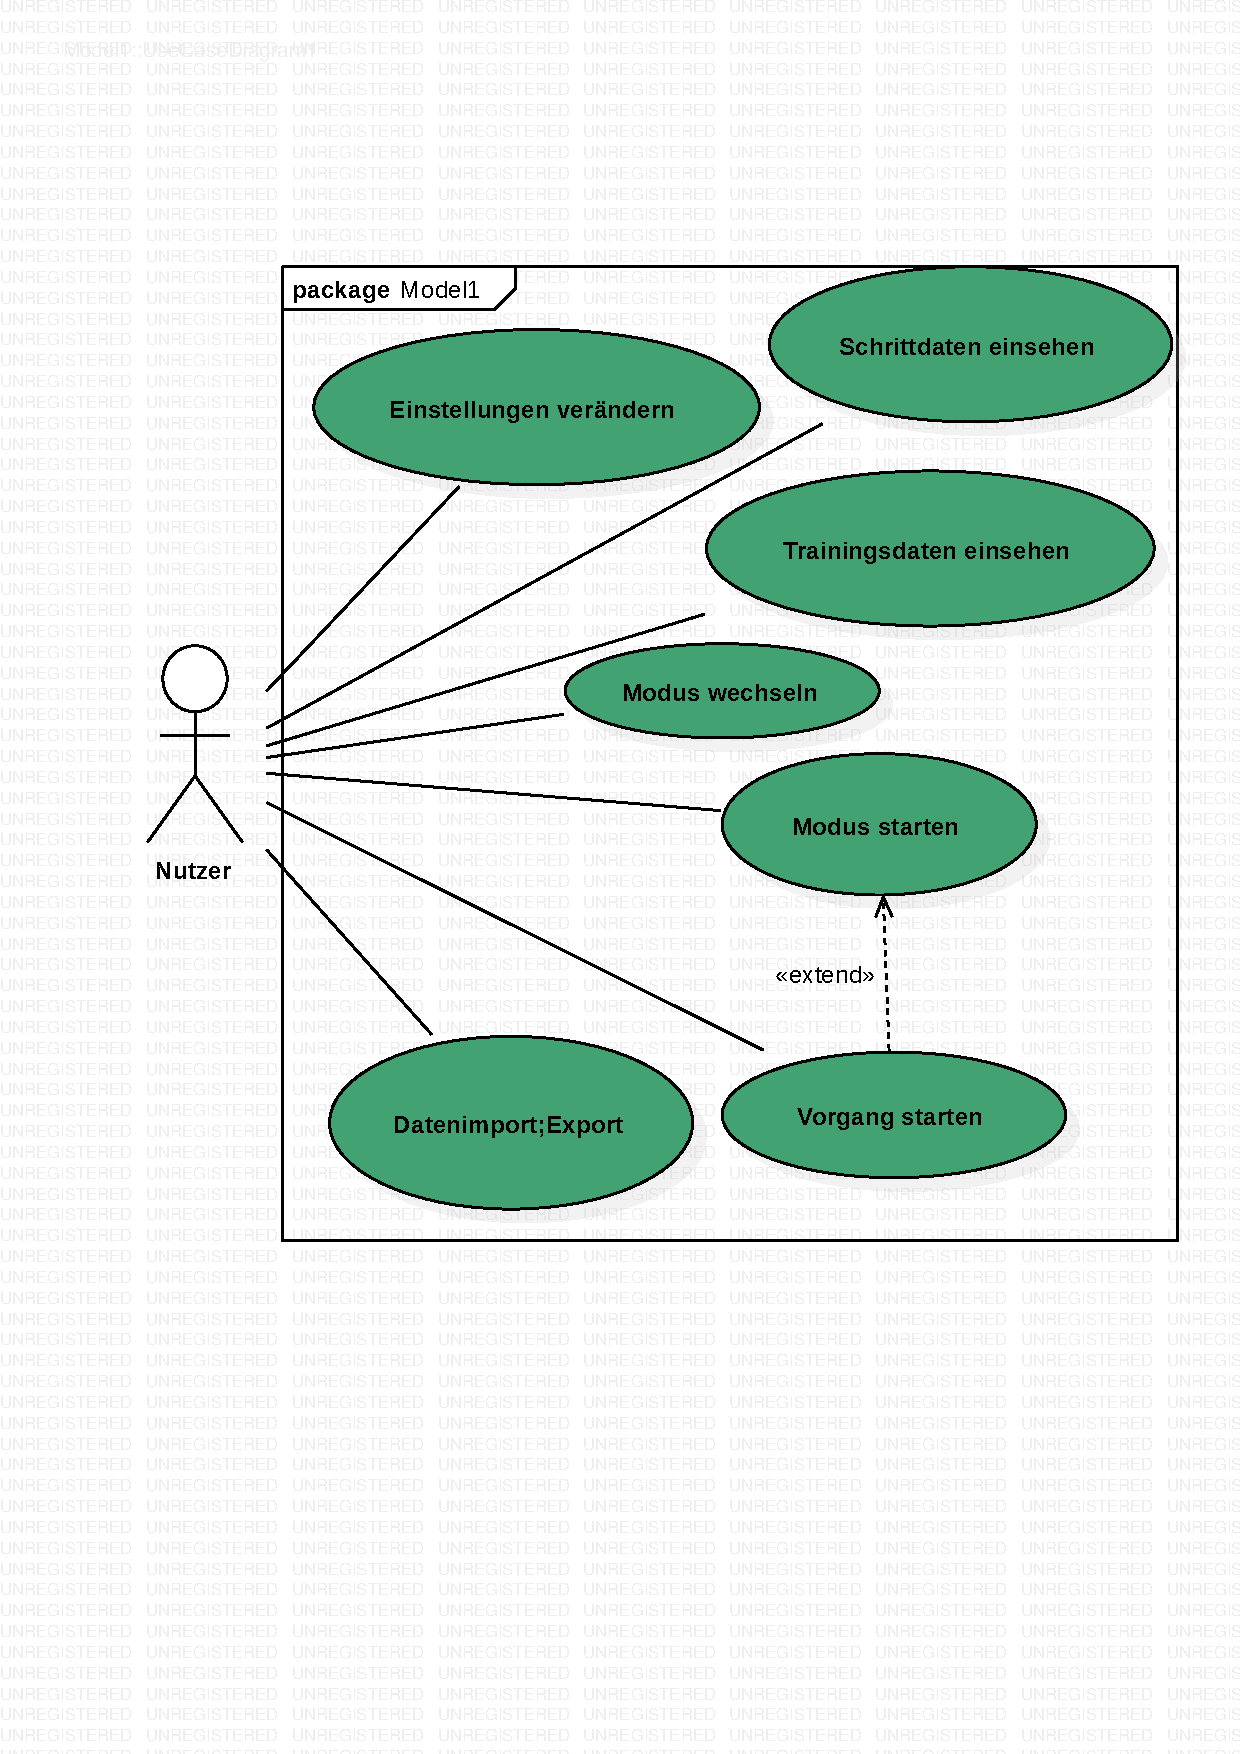
\includegraphics[width=0.8\textwidth]{Vorlaeufiges Use-Case Diagram.pdf}
\end{center}
\section{Benutzeroberfläche}
TODO Benni auseinandersetzen
\section{Qualitätszielbestimmungen} %%Wasn hiermit? Stand noch in der Mail als Unterpunkt. https://www.sosy-lab.org/Teaching/2015-WS-SEP/samples/pflichtenheft.pdf Seite 13 sieht man so eine Tabelle, wie ist das gemeint?
\section{Globale Testfälle und Szenarien}
TODO David
  \subsection{Globale Testfälle}
  \subsubsection{Mussanforderungen}
  \paragraph{Schritterkennung beim Gehen}
  \begin{enumerate}
    \item Das Smartphone wird per Bluetooth mit den Kopfhörern verbunden.
    \item Die App wird gestartet.
    \item Nach dem Startvorgang der App wird in den Modus \glqq Laufmodus\grqq{}(/F100/) gewechselt.
    \item Die Kopfhörer werden korrekt am Ohr des Nutzers angebracht.
    \item Die App zeigt dem Nutzer den Status \glqq stehend\grqq{} an.
    \item Sobald der Nutzer anfängt zu gehen zeigt die App \glqq gehend\grqq{} an.
    \item Sobald der Nutzer wieder still steht ändert sich der Zustand wieder zurück zu \glqq stehend\grqq. 
  \end{enumerate}

  \paragraph{Start/Stop Musikmodus}
  \begin{enumerate}
    \item Das Smartphone wird per Bluetooth mit den Kopfhörern verbunden.
    \item Der Nutzer spielt Musik mit der vorinstallierten Musik-App ab.
    \item Die App wird gestartet.
    \item Nach dem Startvorgang der App wird in den Modus \glqq Start/Stop Musikmodus\grqq{} (/F210/) gewechselt.
    \item Die Kopfhörer werden korrekt am Ohr des Nutzers angebracht.
    \item Der Nutzer beginnt zu gehen.
    \item Der Nutzer startet den gewählten Modus.
    \item Der Nutzer hört auf zu gehen.
    \item Die Musik wird pausiert.
    \item Der Nutzer geht weiter.
    \item Die Musik startet automatisch wieder.
  \end{enumerate}

  
  \subsection{Szenarien}
    \subsubsection{Bibliotheksnutzung}


\section{Entwicklungsumgebung}
TODO valle

Wir arbeiten an dem Projekt mit Visual Studio 2019, sodass alle eine einheitliche Entwicklungsumgebung verwenden.
%%TODO vllt noch mal diskutieren:
Dabei kommt der .NET Standard 2.0 zum Einsatz, der C\# 7.2 verwendet. Wir arbeiten außerdem mit Xamarin Forms.

Zur Versionskontrolle und zur Projektübersicht wird Git verwendet, das Repository liegt öffentlich auf Github\footnote{\url{https://github.com/vlle1/earablesKIT}}.
\clearpage
\newglossaryentry{Echtzeit}{name=Echtzeit, description={Bereitstellen/Anzeigen von Daten mit einer durch die Verarbeitung bedingten Verzögerung von bis zu ca. 2 Sekunden zwischen dem Anfallen der (Roh-)Daten und der Ausgabe bzw. Visualisierung.}}
\newglossaryentry{Vorgang}{name=Vorgang, description={Als Vorgang wird in diesem Pflichtenheft bezeichnet, wenn ein Modus ausgewählt ist und Start gedrückt wurde. Der Vorgang endet mit dem Drücken von Stopp bzw. wird mit dem Wechseln des Modus.}}
\newglossaryentry{BLE}{name=BLE, description={Bluetooth Low Energy ist eine Technologie, die Teil des Industriestandards Bluetooth ist und eine energiesparende, kabellose Kommunikation zwischen Geräten in einer Entfernung von bis zu ca. 10 Metern ermöglicht.}}
\newglossaryentry{Wearable Computer}{name=Wearable Computer, description={Unter dem Begriff Wearable Computer versteht man Computersysteme, die am Körper, unter der Kleidung oder als Implantat unter der Haut getragen werden können.}}
\newglossaryentry{IMU}{name=6-Achsen IMU, description={Ein 6-Achsen IMU ist ein Beschleunigungssensor mit Gyroskop.}}
\newglossaryentry{GUI}{name=GUI, description={GUI ist die Abkürzung für den englischen Begriff \glqq graphical user interface\grqq . Sie ist die Schnittstelle zwischen Mensch und Maschine und ermöglicht dem Nutzer die Eingabe/Steuerung, der Maschine.}}
\newglossaryentry{CPB}{name=Cross-Platform Bibliothek, description={Eine Cross-Platform Bibliothek ist nichts weiter als eine Bibliothek die auf Rechnersystemen mit verschiedener Architektur laufen kann.}}
\newglossaryentry{Steuerungsparameter}{name=Steuerungsparameter, description={Unter Steuerungsparametern fassen wir die Länge der Verbindungsintervalle zwischen Earables und Smartphone sowie die Abtastrate und den Wertebereich von integriertem Gyroskop und Beschleunigungssensor zusammen.}}
\newglossaryentry{Schrittfrequenz}{name=Schrittfrequenz, description={Die Schrittfrequenz gibt an wie viele Schritte pro Zeiteinheit gemacht werden.}}
\newglossaryentry{Rohdaten}{name=Rohdaten, description={Als Rohdaten werden unverarbeitete Daten bezeichnet.}}
\newglossaryentry{TTS}{name=Text-To-Speech, description={Ein Text-to-Speech-System (TTS) (oder Vorleseautomat) wandelt Fließtext in eine akustische Sprachausgabe um. Dabei erfolgt diese auf Deutsch oder auf Englisch, abhängig davon, was als Sprache eingestellt ist.}}
\newglossaryentry{Earables}{name=Earables, description={Eine Zusammenschließung des Wortes Wearable und Earphone. Dabei handelt es sich um Kopfhörer, die mit Sensoren ausgestattet sind.}}
\newglossaryentry{Vorgangsdaten}{name=Vorgangsdaten, description={Daten, die bei der Ausführung eines Vorgangs gespeichert werden (z.B. Schritte, Sit-ups,\dots).}}
\newglossaryentry{Datenbank}{name={Datenbank},
	description={Die Datenbank speichert die Trainingsdaten in Form von DBEntries. Dabei wird die Datenbank von dem Plugin SQLite benutzt.}}
\newglossaryentry{SQLite}{name={SQLite-net-pcl},
	description={SQLite-net-pcl basiert auf dem PlugIn SQLite und ist eine portable Version für die Arbeit mit einer SQLite Datenbank. Dabei ist SQLite eine Erweiterung, mit der man lokale Datenbanken ansprechen und verwalten kann. Dabei bietet die Erweiterung eine lokale Datenbank platformunabhängig gleich anzusprechen. Diese Erweiterung wird für die Speicherung der Trainingsdaten benutz}}
\newglossaryentry{CSV}{name={CSV},
	description={CSV steht für "Comma-Seperated-Value" ein Dateityp, bei dem die Attribute durch ein Komma getrennt werden. Eine Zeile bildet dabei immer einen Eintrag ab. Das Format ist human-readable und veränderbar.}}
\newglossaryentry{Rg.Plugins.Popup}{name={Rg.Plugins.Popup},
	description={Rg.Plugins.Popup ist eine Erweiterung (Plugin), welche es einem ermöglicht Pop-up Fenster zu erstellen und anzuzeigen. Dabei ist das Plugin über den Pluginmanager 'NuGet' einbindbar.}}
\newglossaryentry{DependencyInjection}{name={Microsoft.Extensions.DependencyInjection},
	description={Microsoft.Extensions.DependencyInjection ist eine Erweiterung, welches ermöglicht Komponenten als Services zu registrieren und sie somit abgekapselt und modularer zu betrachten. Mit Klassen, wie der ServiceCollection, oder dem ServiceProvicer, bietet die Erweiterung Microsoft.Extensions.DependencyInjection das Framework.}}
\newglossaryentry{NuGet}{name={NuGet},description={NuGet ist ein Plugin-manager für Visual Studio. Dieser ermöglicht es einem einfach neue Erweiterungen dem Projekt hinzuzufügen. Er kümmert sich um die Kompabitlität und bietet ein Verzeichnis der unterschiedlichen Plug-ins.}}
\newglossaryentry{Bluetooth LE Plugin}{name={Bluetooth LE Plugin for Xamarin},description={Diese Erweiterung ermöglicht es die Verbindung mit den \Gls{Earables} herzustellen. Zudem wird die Kommunikation zwischen Device und \Gls{Earables} geregelt. Von dieser Erweiterung erhalten wir die \Gls{IMU}-Daten.}}
\newglossaryentry{Xamarin.Essentials}{name={Xamarin.Essentials},description={Die Erweiterung Xamarin.Essentials ermöglicht einem, Devicespezifische Services anzusprechen. Benutzt wird hiervon die Funktion TextToSpeech. }}
\newglossaryentry{Xamarin.Plugin.Filepicker}{name={Xamarin.Plugin.Filepicker},description={Die Erweiterung Xamarin.Plugin.Filepicker ergänzt die Funktionalität eines Dateiauswähler. Mit diesem kann man in den Dateimanager des Devices und Dateien auswählen. Gebraucht wird dies beim Importieren und Exportieren der Trainingsdaten.}}

\end{document}
